\documentclass[11pt,a4paper]{article}
\oddsidemargin 0.1 cm \evensidemargin 0.1cm \textwidth 16cm
\textheight24cm
\setlength{\topmargin}{0pt}\setlength{\headsep}{0pt}\pagestyle{empty}

\usepackage{graphicx}
\usepackage{variations}
\usepackage{enumerate}
\usepackage{amssymb}
\usepackage[latin1]{inputenc}  
\usepackage{fontenc}   
\usepackage{amsmath}
\usepackage{amsthm}
\usepackage{amsthm}
\usepackage{xypic}
\usepackage{variations}
%\usepackage{fancyhdr}
%\usepackage{xcolor}
%\usepackage{pstricks-add}
\usepackage[francais]{babel}
%\usepackage[french]{babel}
\newtheorem{defi}{D\'{e}finition}
\newtheorem{thm}{Th\'{e}or\`{e}me}
\newtheorem{rmq}{Remarque}
\newtheorem{prop}{Propri\'{e}t\'{e}}
\newtheorem{prop-def}{Propri\'{e}t\'{e}-D\'{e}finition}
\newtheorem{ex}{Exemple}
\newtheorem{exs}{Exemples}
\newtheorem{exer}{Exercice}
%\newtheorem{proof}{D\'{e}monstration}
\def\di{\displaystyle}
\newcommand{\vtab}{\rule[-0.4em]{0pt}{1.2em}}
\usepackage[top=0.5cm,bottom=0.5cm,right=1.5cm,left=1.5cm]{geometry}
\usepackage{pstricks,pst-plot} 
%\usepackage{framed}
\usepackage{amsmath}
%\usepackage{amssymb}
\usepackage{fancyhdr}
\usepackage{fancybox}
\usepackage{multicol}
%\usepackage{xcolor}
\usepackage{epsfig}
\usepackage{pifont}
%\usepackage[framed]{ntheorem}
%\usepackage[frenchb]{babel}
\usepackage{tabularx}
\def\R{{\mathbb R}}
\newtheorem{Rem}{Remarque}
\newcommand{\V}{\overrightarrow}
\newcommand{\Rep}{(O;\V{\imath};\V{\jmath})}
\newcommand{\Coor}[2]{\begin{pmatrix} #1\\#2 \end{pmatrix}}

\begin{document}
\title{}         % Enter your title between curly braces
\author{}        % Enter your name between curly braces
\date{}          % Enter your date or \today between curly braces
\maketitle

\indent\vspace{-3cm}

$$\fbox{\text{\begin{Large}Chapitre 1 - Feuille d'exercices n�1 : les translations\end{Large}}}$$

\hfill\\[0.2cm]
     

\noindent\underline{\textbf{Exercice 1 :}}\\[-0.8cm]
\begin{minipage}{0.5\linewidth}
\noindent Sur le dessin ci-contre, le triangle $DEF$ est l'image du triangle $ABC$ par une translation. Quelles �galit�s vectorielles peut-on �crire ?
\end{minipage}
\begin{minipage}{0.5\linewidth}
$$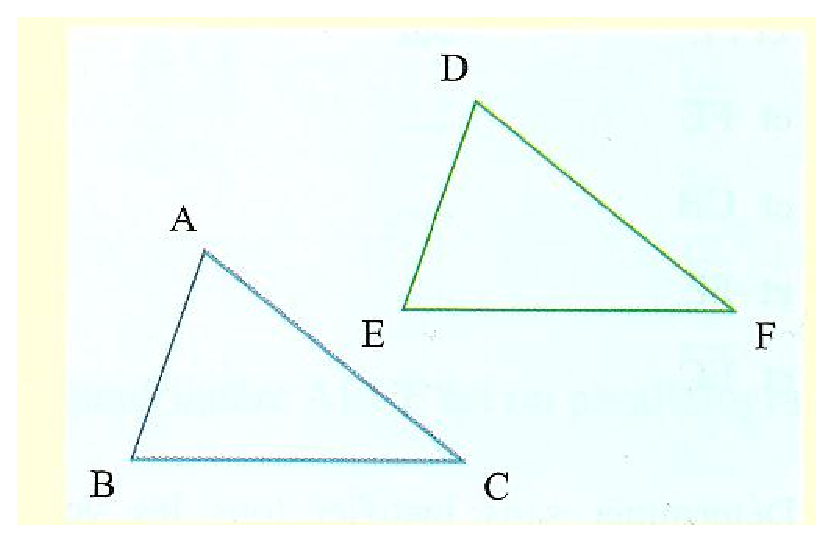
\includegraphics[scale=0.4]{exo1.eps}$$
\end{minipage}
\hfill\\[-0.5cm]

\noindent\underline{\textbf{Exercice 2 :}}\\[0.2cm]
\begin{minipage}{0.6\linewidth}
\noindent On donne la figure ci-contre.
\begin{enumerate}
\item Quelle est l'image du triangle n�$7$ par la translation de vecteur $\V{u}$ ?
\item Quelle est l'image du triangle n�$1$ par la translation de vecteur $\V{u}$ ?
\item Le triangle n�$10$ est l'image du triangle n�$14$ par une translation. Quelle est l'image du triangle n�$13$ par cette m�me translation ?
\item Le triangle n�$10$ est l'image du triangle n�$2$ par une translation. Quelle est l'image du triangle n�$7$ par cette m�me translation ?
\end{enumerate}
\end{minipage}
\begin{minipage}{0.4\linewidth}
$$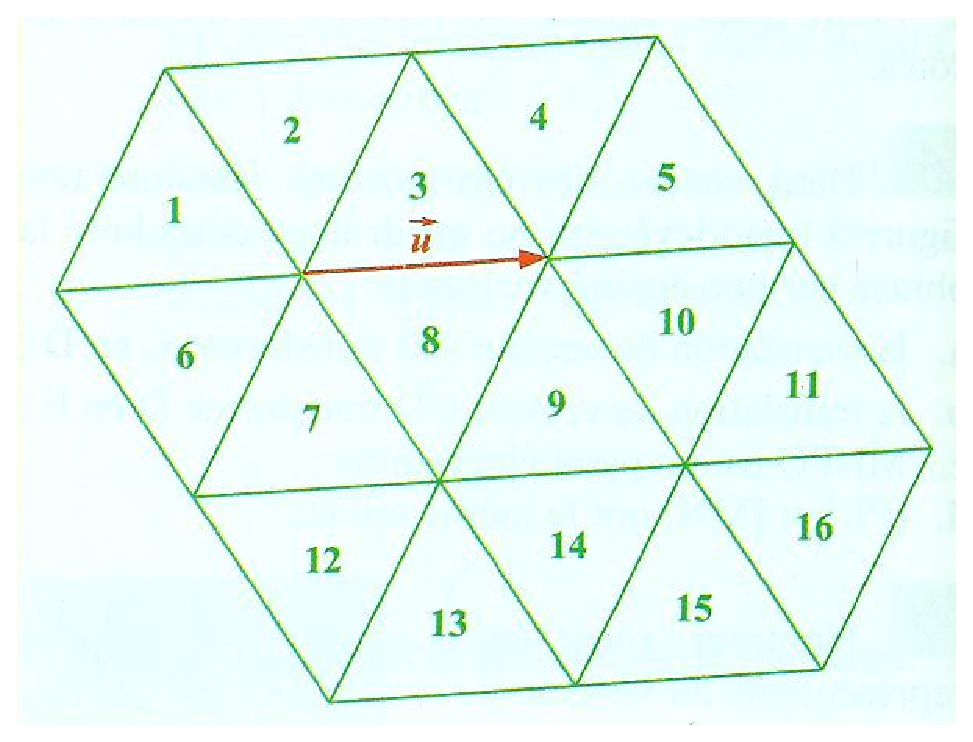
\includegraphics[scale=0.4]{exo2.eps}$$
\end{minipage}
\hfill\\


\noindent\underline{\textbf{Exercice 3 :}}\\[0.2cm]
\begin{minipage}{0.65\linewidth}
On donne la figure ci-contre.
\begin{enumerate}
\item
	\begin{enumerate}[$a.$]
	\item Quelle est l'image du triangle n�$5$ par la translation de vecteur $\V{AB}$ ?
	\item Quelle est l'image du triangle n�$9$ par la translation de vecteur $\V{BC}$ ?
  \item En d�duire l'image du triangle n�$5$ par la compos�e de la translation de vecteur $\V{AB}$ suivie de la translation de vecteur $\V{BC}$. 
	\end{enumerate}
\item Quelle est l'image du triangle n�$5$ par la compos�e de la translation de vecteur $\V{BC}$ suivie de la translation de vecteur $\V{AB}$ ?
\item Quelle �galit� vectorielle peut-on d�duire des questions $1$ et $2$ ?
\end{enumerate}
\end{minipage}
\begin{minipage}{0.35\linewidth}
$$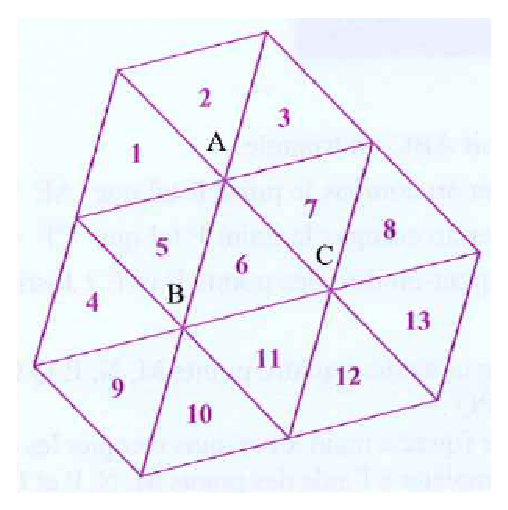
\includegraphics[scale=0.65]{exo3.eps}$$
\end{minipage}
\hfill\\


\noindent\underline{\textbf{Exercice 4 : }}\\[-0.4cm]
\begin{minipage}{0.5\linewidth}
On consid�re la figure ci-contre. $ELUM$ est un parall�logramme. $C$ est le milieu de $[MU]$, $H$ est celui de $[UL]$, $A$ celui de $[EL]$ et $T$ celui de $[EM]$.\\
Quelles �galit�s vectorielles peut-on �crire ?
\end{minipage}
\begin{minipage}{0.5\linewidth}
$$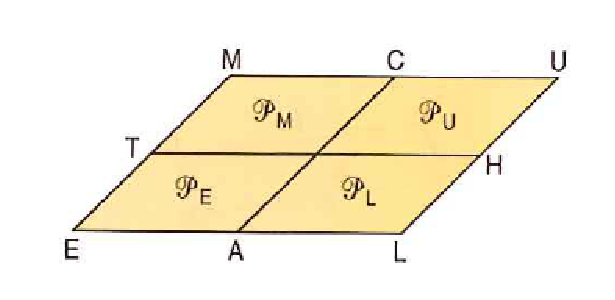
\includegraphics[scale=0.6]{exo4.eps}$$
\end{minipage}


\noindent\underline{\textbf{Exercice 5 : Vrai ou faux ?}}\\[0.2cm]
Si $\V{AB}=\V{CD}$, alors :
\begin{enumerate}[$\diamond$]
\item $D$ est l'image de $C$ par la translation de vecteur $\V{AB}$ ;
\item $B$ est l'image de $A$ par la translation de vecteur $\V{CD}$ ;
\item $\V{AD}=\V{BC}$ ;
\item $C$ est l'image de $A$ par la translation de vecteur $\V{BD}$ ;
\item $ABCD$ est un parall�logramme.
\end{enumerate}
\hfill\\








\end{document}
